\setlength{\columnsep}{3pt}
\begin{flushleft}
	Commands to display process related details:
	\begin{itemize}
		\item \textbf{ps}: Display current processes.
		\bigskip
		\begin{tcolorbox}[breakable,notitle,boxrule=-0pt,colback=pink,colframe=pink]
			\color{black}
			\fontdimen2\font=1em
			Syntax: ps [options]
			\fontdimen2\font=4pt
		\end{tcolorbox}
		Eg: \textbf{ps} command without any option display current terminal process.
		\begin{tcolorbox}[breakable,notitle,boxrule=-0pt,colback=black,colframe=black]
			\color{green}
			\fontdimen2\font=1em
			\#  ps
			\color{white}
			\newline
			    PID TTY          TIME CMD
			\newline
			190566 pts/3    00:00:00 bash
			\newline
			190577 pts/3    00:00:00 bc
			\newline
			197680 pts/3    00:00:00 ps
			\fontdimen2\font=4pt
		\end{tcolorbox}
		
		Options with \textbf{ps} command:	
		
		
		\begin{itemize}
			\item \textbf{Display all process running in all terminals by all user.}
			\bigskip
			\begin{tcolorbox}[breakable,notitle,boxrule=-0pt,colback=pink,colframe=pink]
				\color{black}
				\fontdimen2\font=1em
				Syntax: ps -aux
				\fontdimen2\font=4pt
			\end{tcolorbox}	
			where,
			\newline
			\textbf{-a}: List all processes with a terminal (tty).
			\newline
			\textbf{-x}: List all processes owned by all users.
			\newline
			\textbf{-u}: Display user-oriented format.
			\newline
			Eg: 
			\begin{figure}[h!]
				\centering
				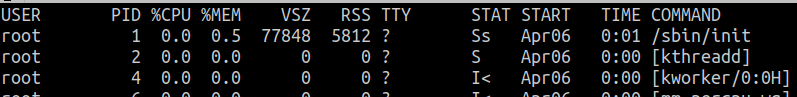
\includegraphics[scale=.35]{content/chapter12/images/ps.png}
				\caption{Sample output}
				\label{fig:process234}
			\end{figure}
			\newline
			Output explaination:
			\begin{itemize}
				\item \textbf{USER}: User owning the process
				\item \textbf{PID}: Process ID
				\item \textbf{\%CPU}: CPU utilisation
				\item \textbf{\%MEM}: Memory utilisation
				\item \textbf{RSS}: The resident set size, the non-swapped physical memory that the process has used in kilobytes
				\item \textbf{VSZ}: Gives the virtual size of the process, code, data and stack segments
				\item \textbf{TTY}: 
				\begin{itemize}
					\item Terminal on which the process is running
					\item \textbf{"?"} means process is running in background
				\end{itemize}
				\item \textbf{STAT}: Display process state as shown below:
					\newline
					 Process states:
					\begin{itemize}
						\item \textbf{D}: Uninterruptible sleep (usually IO)
						\item \textbf{I}: Idle kernel thread
						\item \textbf{R}: Running process
						\item \textbf{S}: Interruptible sleep (waiting for an event to complete)
						\item \textbf{T}: Stopped process
						\item \textbf{t}: Stopped by debugger during the tracing
						\item \textbf{X}: Dead (should never be seen)
						\item \textbf{Z}: Defunct ("zombie") process, terminated but not reaped by
						its parent
					\end{itemize}
					Additional characters:
					\begin{itemize}
						\item \textbf{<}: High-priority
						\item \textbf{+}: Foreground process
						\item \textbf{N}: Low-priority
						\item \textbf{s}: Session leader
						\item \textbf{L}: Has pages locked into memory
						\item \textbf{l}: Multi-threaded process
					\end{itemize}
					\item \textbf{START}: Start time of process
					\item \textbf{TIME}: How long the process takes to execute
					\item \textbf{COMMAND}: Program in running state
			\end{itemize}
			
			\newpage
			
			\item \textbf{Display all processes along with it's parent process ID (PPID).}
		
			\begin{tcolorbox}[breakable,notitle,boxrule=-0pt,colback=pink,colframe=pink]
				\color{black}
				\fontdimen2\font=1em
				Syntax: ps -ef
				\fontdimen2\font=4pt
			\end{tcolorbox}	
			where,
			\newline
			\textbf{-e}: Display all the processes.
			\newline
			\textbf{-f}: Display full format listing along with PPID (i.e parent process ID).
			\newline
			Eg:
			\begin{figure}[h!]
				\centering
				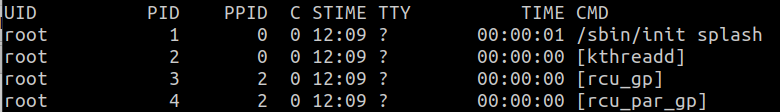
\includegraphics[scale=.4]{content/chapter12/images/ps2.png}
				\caption{Sample output}
				\label{fig:process2348}
			\end{figure}
		
			\bigskip
			\bigskip
			
			\item \textbf{Display all process related to a specific user.}
			\bigskip
			\begin{tcolorbox}[breakable,notitle,boxrule=-0pt,colback=pink,colframe=pink]
				\color{black}
				\fontdimen2\font=1em
				Syntax: ps -u user\_name
				\fontdimen2\font=4pt
			\end{tcolorbox}	
			where,
			\newline
			\textbf{-u}: Display all process related to a specific user.
			\newline
			Eg:
			\begin{figure}[h!]
				\centering
				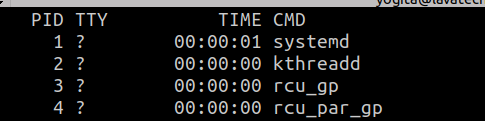
\includegraphics[scale=.6]{content/chapter12/images/ps3.png}
				\caption{Sample output}
				\label{fig:process2345}
			\end{figure}
		\newpage
		
		
		\item \textbf{Find all process of a specific process name.}
		\bigskip
		\begin{tcolorbox}[breakable,notitle,boxrule=-0pt,colback=pink,colframe=pink]
			\color{black}
			\fontdimen2\font=1em
			Syntax: ps -C process\_name
			\fontdimen2\font=4pt
		\end{tcolorbox}	
		where,
		\newline
		\textbf{-C}: Display all process related to a specific process name.
		\newline
		Eg:
		\begin{figure}[h!]
			\centering
			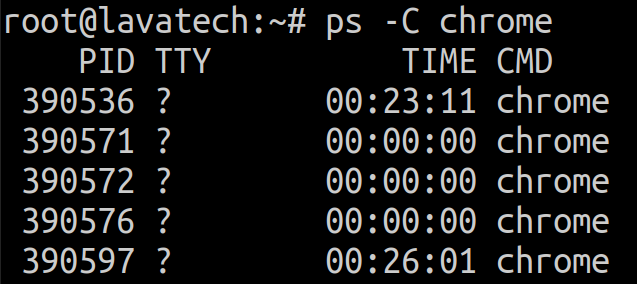
\includegraphics[scale=.4]{content/chapter12/images/ps_u.png}
			\caption{Sample output}
			\label{fig:process23454}
		\end{figure}
			
		\bigskip
		\bigskip
		
		\item \textbf{Find process name of a specific process ID (PID).}
		\bigskip
		\begin{tcolorbox}[breakable,notitle,boxrule=-0pt,colback=pink,colframe=pink]
			\color{black}
			\fontdimen2\font=1em
			Syntax: ps -f -p  PID
			\fontdimen2\font=4pt
		\end{tcolorbox}	
		where,
		\newline
		\textbf{-p}: Display all process related to a PID.
		\newline
		\textbf{-f}: Display full detailed information.
		\newline
		Eg:
		\begin{figure}[h!]
			\centering
			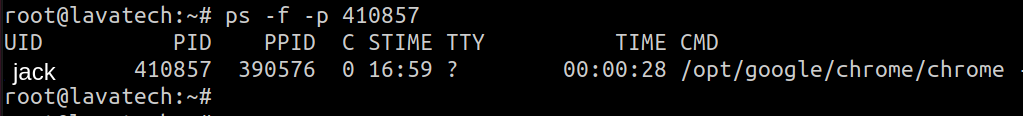
\includegraphics[scale=.3]{content/chapter12/images/ps_p.png}
			\caption{Sample output}
			\label{fig:process234549}
		\end{figure}
							
		\end{itemize}
	
	\newpage
	\item \textbf{pstree} - Display a tree of processes.
	\bigskip
	\begin{tcolorbox}[breakable,notitle,boxrule=-0pt,colback=pink,colframe=pink]
		\color{black}
		\fontdimen2\font=1em
		Syntax: pstree
		\fontdimen2\font=4pt
	\end{tcolorbox}
	
	Eg:
	\begin{figure}[h!]
		\centering
		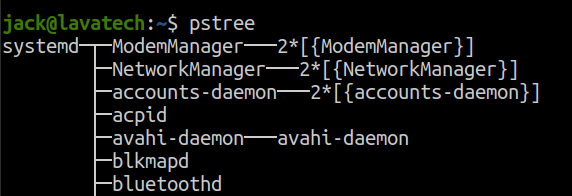
\includegraphics[scale=.4]{content/chapter12/images/pstree.png}
		\caption{Sample output}
		\label{fig:process2345492}
	\end{figure}
	Option with \textbf{pstree} command:
	\newline
	\textbf{-u}: Display all process related to a specific user.
	\bigskip
	\begin{tcolorbox}[breakable,notitle,boxrule=-0pt,colback=pink,colframe=pink]
		\color{black}
		\fontdimen2\font=1em
		Syntax: pstree -u username
		\fontdimen2\font=4pt
	\end{tcolorbox}
	
	Eg:
	\begin{tcolorbox}[breakable,notitle,boxrule=-0pt,colback=black,colframe=black]
		\color{green}
		\fontdimen2\font=1em
		\# pstree -u jack
		\fontdimen2\font=4pt
	\end{tcolorbox}
	
	
	\bigskip
	\bigskip
	
	\item \textbf{fuser}: Find PID of running process accessing specific file/directory.
	\bigskip
	\begin{tcolorbox}[breakable,notitle,boxrule=-0pt,colback=pink,colframe=pink]
		\color{black}
		\fontdimen2\font=1em
		Syntax: fuser -v file\_folder
		\fontdimen2\font=4pt
	\end{tcolorbox}

	Eg:
	\begin{figure}[h!]
		\centering
		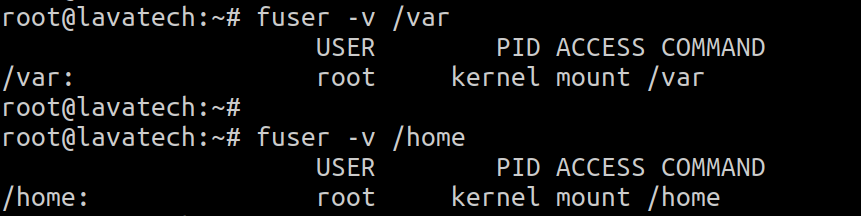
\includegraphics[scale=.4]{content/chapter12/images/fuser.png}
		\caption{Sample output}
		\label{fig:process2345492}
	\end{figure}
	
	\bigskip
	\bigskip
	
	\item \textbf{pidof}: Find PID of all running process using the process name.
	\bigskip
	\begin{tcolorbox}[breakable,notitle,boxrule=-0pt,colback=pink,colframe=pink]
		\color{black}
		\fontdimen2\font=1em
		Syntax: pidof process\_name
		\fontdimen2\font=4pt
	\end{tcolorbox}
	
	Eg:
	\begin{figure}[h!]
		\centering
		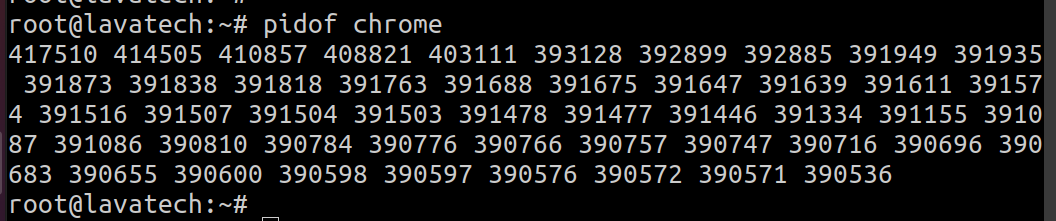
\includegraphics[scale=.35]{content/chapter12/images/pidof.png}
		\caption{Sample output}
		\label{fig:process23454922}
	\end{figure}
	
	
	\newpage
	
	\item \textbf{top}: Displays real time process with CPU load, memory usage etc.
	\bigskip
	\begin{tcolorbox}[breakable,notitle,boxrule=-0pt,colback=pink,colframe=pink]
		\color{black}
		\fontdimen2\font=1em
		Syntax: top
		\fontdimen2\font=4pt
	\end{tcolorbox}

	Eg:	
	\bigskip
	\begin{figure}[h!]
		\centering
		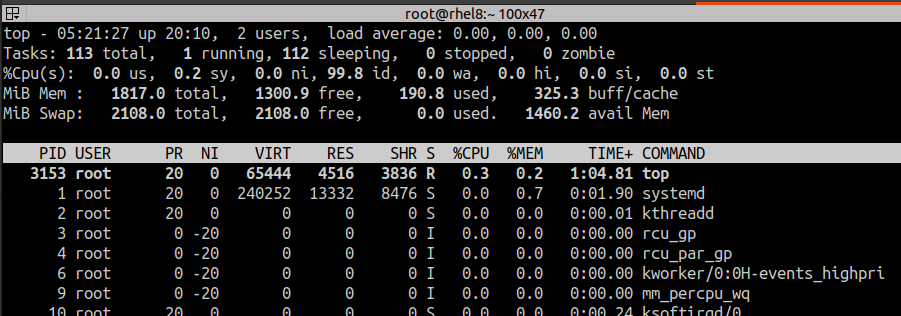
\includegraphics[scale=0.4]{content/chapter12/images/top_command.png}
		\caption{Top command output}
		\label{fig:top_command_output}
	\end{figure}
	Press \textbf{"CTRL+C" or "q"} to exit from the command output.
	
	\newline
	\bigskip
	Options with \textbf{top} command:
	\newline
	\textbf{-u}: Display all process of specific user.
	\bigskip
	\begin{tcolorbox}[breakable,notitle,boxrule=-0pt,colback=pink,colframe=pink]
		\color{black}
		\fontdimen2\font=1em
		Syntax: top -u username
		\fontdimen2\font=4pt
	\end{tcolorbox}
	
	Eg: \textbf{top} command to display all process associated with \textbf{"root"} user.
	\begin{tcolorbox}[breakable,notitle,boxrule=-0pt,colback=black,colframe=black]
		\color{green}
		\fontdimen2\font=1em
		\#  top -u root
		\fontdimen2\font=4pt
	\end{tcolorbox}
		
		
	\end{itemize}

\end{flushleft}

\newpage


